%%This is a very basic article template.
%%There is just one section and two subsections.
\documentclass{jarticle}
\usepackage[top=20truemm,bottom=15truemm,left=20truemm,right=20truemm]{geometry}
\usepackage{jlisting, listings, here}
\usepackage[dvipdfmx]{graphicx}
\makeatletter
\def\maketitle{%
\null
\thispagestyle{empty}%
\vfill
\begin{center}\leavevmode
\normalfont
{\LARGE \@title\par}%
\vskip 1cm
{\Large \@author\par}%
\vskip 1cm
{\Large \@date\par}%
\end{center}%
\vfill
\null
\@thanks%\vfil\null
\cleardoublepage
}
\makeatother
\lstset{language=c,
basicstyle=\ttfamily\scriptsize,
commentstyle=\textit,
classoffset=1,
keywordstyle=\bfseries,
frame=tRBl,
framesep=5pt,
showstringspaces=false,
stepnumber=1,
numberstyle=\tiny,
tabsize=2,
numbers = left,
stepnumber=1
}
\title{ソフトウェア演習V 課題1(再々提出)}
\author{15122013 尾持涼介}
\date{提出日:2017年12月25日}

\begin{document}
\maketitle

\section{作成したプログラムの設計情報}
\subsection{全体構成}
各ファイルで記述した関数は以下の通りである。
\begin{itemize}
  \item token-list.c
  \begin{itemize}
    \item main関数
    \item void error(char *mes)
  \end{itemize}
  \item scan.c
  \begin{itemize}
    \item int keyword\_search(char *string)
    \item int init\_scan(char *filename)
    \item int keyword\_search(char *string)
    \item int scan()
    \item int get\_linenum()
    \item void end\_scan()
  \end{itemize}
  \item id-list.c
  \begin{itemize}
    \item void init\_idtab()
    \item struct ID *search\_idtab(char *np)
    \item void id\_countup(char *np)
    \item void print\_idtab()
    \item void release\_idtab()
  \end{itemize}
\end{itemize}

次に、各関数の呼び出し関係、データ参照関係について述べる。
\begin{itemize}
  \item token-list.c
  \begin{itemize}
    \item main関数内
    \begin{itemize}
      \item init\_scan()関数を呼び出し
      \item scan()関数を呼び出し
      \item end\_scan()関数を呼び出し
      \item print\_idtab()関数を呼び出し
    \end{itemize}
    \item error関数内
    \begin{itemize}
      \item get\_linenum()関数を参照
    \end{itemize}
  \end{itemize}
  \item scan.c
  \begin{itemize}
    \item init\_scan()関数内
    \begin{itemize}
      \item init\_idtab()関数を呼び出し
    \end{itemize}
    \item keyword\_search()関数内
    \begin{itemize}
      \item id\_countup()を呼び出し
    \end{itemize}
    \item scan()関数内
    \begin{itemize}
      \item keyword\_search()関数を呼び出し
    \end{itemize}
  \end{itemize}
  \item id-list.c
  \begin{itemize}
    \item id\_countup()関数内
    \begin{itemize}
      \item search\_idtab()関数を呼び出し
    \end{itemize}
    \item release\_idtab()関数内
    \begin{itemize}
      \item init\_idtab()関数を呼び出し
    \end{itemize}
  \end{itemize}
\end{itemize}
\subsection{各モジュールごとの構成}
キーワードとそのトークンコードを格納するために以下の図\ref{struct-key}のような構造体をヘッダファイルtoken-list.hで定義した。
\begin{figure}[H]
\begin{center}
\begin{lstlisting}
extern struct KEY {
char * keyword;
int keytoken;
} key[KEYWORDSIZE];
\end{lstlisting}
\caption{キーワードとそのトークンコードを格納する構造体}
\label{struct-key}
\end{center}
\end{figure}
また、名前を識別するための構造体を以下の図\ref{struct-id}のような構造体をid-list.c内で定義した。
\begin{figure}[H]
\begin{center}
\begin{lstlisting}
struct ID {
char *name;
int count;
struct ID *nextp;
}  *idroot;
\end{lstlisting}
\caption{名前を識別するための構造体}
\label{struct-id}
\end{center}
\end{figure}

scan.cでは、ctype.hをインクルードし、scan()関数内でcbufに読み込んだ文字がアルファベットかを判別するisalpha()関数、数字、または
アルファベットかどうかを判別するisalnum()関数、数字かどうかを判別するisdigit()関数を使用している。それらを用いてif文で
キーワードあるいは名前、符号なし数字を判別し、その他の記号等はswitch文を用いて判別している。

次に使用した大域変数とその意味について述べる。

\begin{itemize}
  \item token-list.c内
  \begin{itemize}
    \item int
    numtoken[NUMOFTOKEN+1]:各トークンを数え上げるために使用。各トークンのトークンコードと同じ場所にその個数を格納する。すなわち、例えば、
    numtoken[1]には名前の個数が格納される。なお、NUMOFTOKENとは定義したトークンの個数であり、49と定義されている。
    \item char *tokenstr[NUMOFTOKEN+1] :各トークン名が格納されている。
  \end{itemize}
  \item scan.c内
  \begin{itemize}
    \item int cbuf:ファイルから読み込んだ文字を格納する1文字分の文字バッファ
    \item int line\_cnt:行数を数え上げる変数
    \item int newline:次の文字から新しい行が始まる場合は0、そうでない場合は1を格納しておく。
    \item FILE *fp:ファイルを操作するためのポインタ
  \end{itemize}
  \item id-list.c内
  \begin{itemize}
    \item struct ID *idroot:各「名前」とその個数を格納する線形リストの先頭要素を指すポインタ
  \end{itemize}

  次に各関数内で定義した変数とその意味について述べる

  \begin{itemize}
    \item token-list.c
    \begin{itemize}
      \item main関数内
      \begin{itemize}
        \item int token:scan()関数から返却されたトークンコードを格納する。
        \item int i:for文によるループで用いる変数
      \end{itemize}
    \end{itemize}
    \item scan.c
    \begin{itemize}
      \item ikeyword\_search()関数内
      \begin{itemize}
        \item int l:二分探索において左端を指す変数
        \item int r:二分探索において右端を指す変数
        \item int c:二分探索において真ん中を指す変数
        \item int comp:文字列を比較する際に用いるstrcmp()関数からの返り値を格納する変数
      \end{itemize}
      \item scan()関数内
      \begin{itemize}
        \item int num\_attr:scan()の返り値が「符号なし整数」の時、その値を格納する変数。
        \item char
        string\_attr[MAXSTRSIZE]:scan()の返り値が「名前」または「文字列」の時、その実際の文字列を格納する配列。また、それが「符号なし整数」の時は、入力された数字列を格納する。また、MAXSTRSIZEとはこの配列に格納できる文字列の最大長であり、1024と定義している。
        \item int i:string\_attrに文字、または数字を格納していくときにその配列の何番目の要素に格納するかを指定する変数。
      \end{itemize}
    \end{itemize}
    \item id-list.c
    \begin{itemize}
      \item search\_idtab()関数内
      \begin{itemize}
        \item struct ID *p:for文により構造体を探索する際に構造体を操作するポインタ。
      \end{itemize}
      \item id\_countup()関数内
      \begin{itemize}
        \item struct ID
        *p:探索した結果既にその「名前」が構造体に格納されている場合は、その場所を指すポインタとなり、探索した結果初出の名前であった場合は構造体に格納するための情報を格納する新たな要素となる。
        \item char *cp:search\_idtab()関数で探索した「名前」がその初出のものである場合、その「名前」を格納するポインタとなる。
      \end{itemize}
      \item print\_idtab()関数内
      \begin{itemize}
        \item struct ID *p:for文において構造体を操作するためのポインタ
      \end{itemize}
      \item release\_idtab()関数内
      \begin{itemize}
        \item struct ID *p, *q:どちらもfor文において構造体を操作するために使用するポインタ
      \end{itemize}
    \end{itemize}
  \end{itemize}
\end{itemize}
\subsection{各関数の外部(入出力)仕様}
ここでは、各関数の機能、引数と返り値等について説明する。
\subsubsection{token-list.c内で記述されている関数}
\begin{itemize}
  \item main関数
  \begin{description}
\item[引数]コマンドライン引数としてint ncとchar
*np[]を指定する。ncは指定された引数の個数を表し、npはプログラムを起動するときに指定する引数であり、本プログラムでは読み込むファイル名を指定する。
\item[返り値]プログラムが終了した際に0を返す。
\item[参照する大域変数]tokenstr
\item[変更する大域変数]numtoken
\end{description}
\item void error(char *mes)
\begin{description}
\item[機能]エラーが発生したときにエラーメッセージとエラー発生箇所を表示する。
\item[引数]char *mes:表示するエラーメッセージ
\item[返り値]なし
\item[参照・変更する大域変数]なし
\end{description}
\end{itemize}
\subsubsection{scan.c内で記述されている関数}
\begin{itemize}
  \item int init\_scan(char *filename)
  \begin{description}
\item[機能]filenameが表すファイルを入力ファイルとしてオープンする。また、変数line\_cntとnewlineを0に初期化し、cbufに1文字読み込んでおく。
\item[引数]char *filename:開くファイル名
\item[返り値]正常にファイルが開けた場合は0、ファイルが開けなかった場合など異常な場合は-1を返す
\item[参照・変更する大域変数]line\_cnt、newline、cbuf
\end{description}
\item int keyword\_search(char *string)
\begin{description}
\item[機能]読み込んだ文字列がキーワードかどうかを調べる。
\item[引数]char *string:探索する文字列
\item[返り値]探索した結果のトークンコードを返却する。
\item[参照・変更する大域変数]なし
\end{description}
\item int scan()
\begin{description}
\item[機能]トークンを1つスキャンし、そのトークンを識別する。
\item[引数]なし
\item[返り値]トークンのコードを返す。End-of-Fileが現れたときやエラーが発生したときは-1を返す。
\item[参照する大域変数]cbuf、newline、fp
\item[変更する大域変数]cbuf、newline、line\_cnt
\end{description}
\item int get\_linenum()
\begin{description}
\item[機能]最も最近にscan()で返されたトークンが存在した行番号を返す関数。
\item[引数]なし
\item[返り値]最も最近にscan()で返されたトークンが存在した行番号を返す。まだ一度もscan()が呼ばれていないときには0を返す。
\item[参照・変更する大域変数]なし
\end{description}
\item void end\_scan()
\begin{description}
\item[機能]init\_scan()関数でオープンしたファイルをクローズする。
\item[引数・返り値]なし
\item[参照・変更する大域変数]fp
\end{description}
\end{itemize}
\subsubsection{id-list.c内で記述した関数}
\begin{itemize}
  \item void init\_idtab()
  \begin{description}
\item[機能]名前を識別するための構造体を初期化する。
\item[引数・返り値]なし
\item[変更する大域変数]idroot
\end{description}
\item struct ID *search\_idtab(char *np)
\begin{description}
\item[機能]指定された「名前」が線形リスト内に存在するかを探索する。
\item[引数]char *np:探索する「名前」
\item[返り値]探索した結果その「名前」が線形リスト内に発見されればその要素を指すポインタ、もし見つからなければNULLを返す。
\item[参照する大域変数]idroot
\end{description}
\item void id\_countup(char *np)
\begin{description}
\item[機能]npで指定された名前の個数を数え上げる。
\item[引数]char *np:数え上げる「名前」
\item[返り値]なし
\item[参照・変更する大域変数]idroot
\end{description}
\item void print\_idtab()
\begin{description}
\item[機能]各「名前」とその個数を表示する。
\item[引数・返り値]なし
\item[参照する大域変数]idroot
\end{description}
\item void release\_idtab()
\begin{description}
\item[機能]idrootが確保していた領域を解放する。
\item[引数・返り値]なし
\item[参照・変更する大域変数]idroot
\end{description}
\end{itemize}
\section{テスト情報}
\subsection{テストデータ・テスト結果}
私はまず、ブラックボックステストとして配布されたテストデータである、sample011.mpl、sample014.mpl、sample11.mpl、sample11p.mpl、sample11pp.mpl、sample12.mpl、
sample13.mpl、sample14.mpl、sample15.mpl、sample15a.mpl、sample16.mpl、sample17.mpl、sample18.mpl、
sample19p.mplについてテストを行った。さらに、ホワイトボックステストとしてmysample01.mpl、mysample02.mpl、mysample03.mpl、
mysample04.mpl、mysample05.mpl、mysample06.mpl、mysample07.mpl、mysample08.mplというテストデータを用意してテストを行った。

配布されたテストデータによるテスト結果と、mysample05.mpl以外の自作のテストデータとその結果についてはメールにより提出する。
なお、テスト結果を格納するファイル名は「(テストプログラム名)\_test.txt」としている(テストプログラム名の.mplは省略)。それらをまとめて「kadai1-test.zip」
というファイルにまとめて圧縮して提出する。テスト結果を格納しているファイルには
想定される出力結果と、実際に行ったテスト結果が書き込まれており、「想定」以下が想定される出力結果で、「結果」以下が
実際の出力結果である。テスト情報を添付したメールの送信日時は11月27日10時08分である。

mysample05.mplについては以下で説明する。このファイルは何も書き込まれていない空ファイルである。すなわちファイルから1文字読み込むと
いきなりEOFが現れるファイルである。このファイルを用いてテストを行ったところ、標準出力には何も表示されないままプログラムは終了した。
なお、これは想定通りの動作である。
\subsection{テストデータの十分性}
改行コードについては環境によって4通りのうちどれが現れるかは決まるので、以下では4通りのうちどれかが出現したら「改行コードに関する命令は
網羅された」として議論する。

sample014.mpl以外の配布されたテストデータとmysample05.mplで、エラーメッセージが表示されない場合に通るすべての命令が網羅されている。

残りのテストデータにおいて通常実行されない、コマンドラインが与えられていないときのエラーメッセージ、ファイルが開けないときのエラーメッセージが
表示される場合を除く、エラーメッセージを表示するすべての場合に通る命令を網羅している。

\section{本課題を行うための事前計画(スケジュール)と実際の進捗状況}
\subsection{事前計画(スケジュール)}
事前計画は以下の表\ref{tb:jizen}のように立てた。
\begin{table}[H]
\begin{center}
\caption{課題1における事前計画}
\label{tb:jizen}
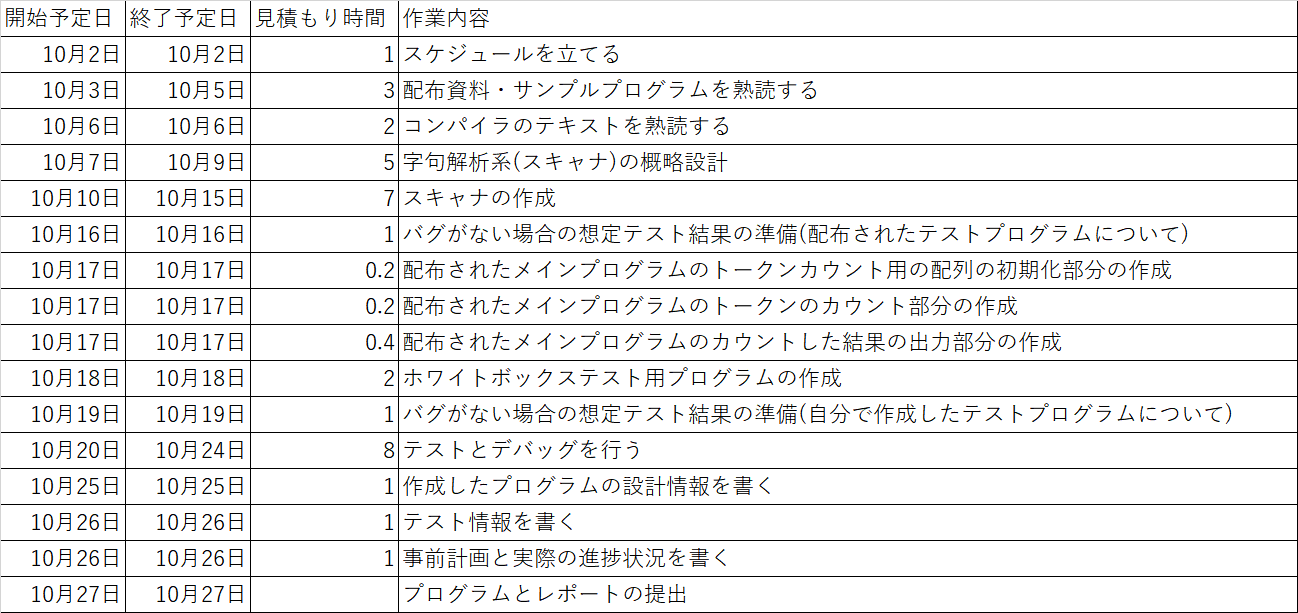
\includegraphics[scale=0.6]{kadai1.png}
\end{center}
\end{table}

しかし、演習中に計画を以下の表\ref{tb:shusei}のように修正した。
\begin{table}[H]
\begin{center}
\caption{課題1における修正後のスケジュール}
\label{tb:shusei}
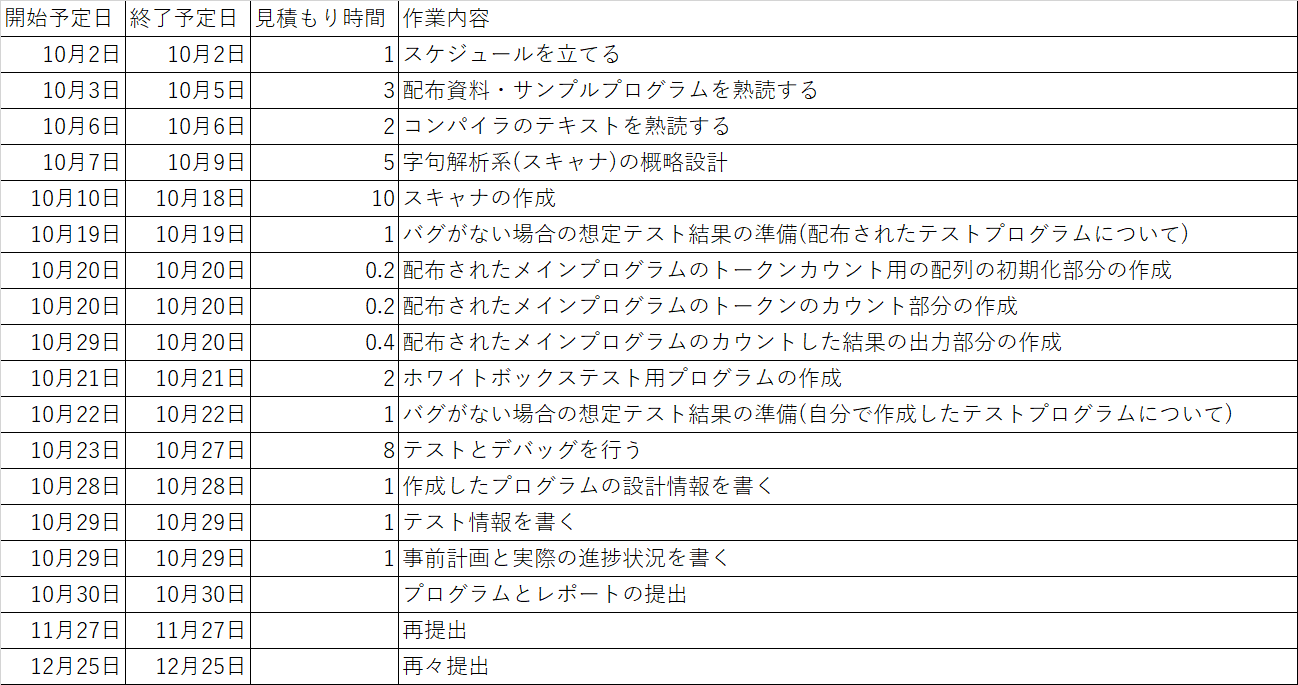
\includegraphics[scale=0.6]{kadai1-2.png}
\end{center}
\end{table}
\subsection{実際の進捗状況}
表\ref{tb:shusei}のように変更したように、スキャナのコーディングが予想以上に時間がかかってしまった。その他の作業については
だいたい計画通りに進んだ。

しかし、課題2に取り組んでいる際にscan.c内に誤りを見つけたため再提出を行った。また、keyword\_search()関数において、不必要な関数を呼び出していたので、再々提出を行った。
\subsection{当初の事前計画と実際の進捗との差の原因}
配布資料・プログラムやテキストの熟読が十分でなく、理解不足であったことが原因であると考えられる。そのため、コーディングの際にも
何度もテキストや配布資料を読むこととなり、余計に時間がかかってしまったのである。このようなことをなくすために、次回以降は
テキストや配布資料を熟読する時間を長めにとるようにすればよいと考えられる。また、再提出となったのは、見直しが不十分であったからであると考えられる。
\end{document}
